\documentclass[aps,letterpaper,11pt]{revtex4}
\usepackage{graphicx} % For images
\usepackage{float}    % For tables and other floats
\usepackage{verbatim} % For comments and other
\usepackage{amssymb}  % For more math
\usepackage{fullpage} % Set margins and place page numbers at bottom center
\usepackage{listings} % For source code
\usepackage[usenames,dvipsnames]{color} % For colors and names
\usepackage[pdftex]{hyperref}           % For hyperlinks and indexing the PDF
\usepackage{pdfpages}
\usepackage{subfig}
\usepackage{listings}
\usepackage[usenames,dvipsnames,svgnames,table]{xcolor}
\usepackage{color}
\usepackage{textcomp}
\usepackage[utf8]{inputenc}
% Custom colors
\definecolor{deepblue}{rgb}{0,0,0.5}
\definecolor{deepred}{rgb}{0.6,0,0}
\definecolor{deepgreen}{rgb}{0,0.5,0}

 \lstset{
  tabsize=4,
  language=C++,
  captionpos=b,
  tabsize=3,
  numberstyle=\tiny,
  numbersep=5pt,
  breaklines=true,
  showstringspaces=false,
  basicstyle=\footnotesize,
%  identifierstyle=\color{magenta},
  keywordstyle=\color[rgb]{0,0,1},
  commentstyle=\color{deepgreen},
  stringstyle=\color{deepred}
  }
  
\hypersetup{ % play with the different link colors here
    colorlinks,
    citecolor=black,
    filecolor=black,
    linkcolor=black,
    urlcolor=blue % set to black to prevent printing blue links
}

\newcommand{\labno}{Technical report}
\newcommand{\labtitle}{Image Pixelization}
\newcommand{\authorname}{Antoine Merlet}
\newcommand{\professor}{Dr. Yohan Fougerolle}


\begin{document}  
\begin{titlepage}
\begin{center}
{\LARGE \textsc{\labno:} \\ \vspace{4pt}}
{\Large \textsc{\labtitle} \\ \vspace{4pt}} 
\rule[13pt]{\textwidth}{1pt} \\ \vspace{150pt}
{\large By: \authorname \\ \vspace{10pt}
Professor: \professor \\ \vspace{10pt}
\today}
\end{center}




\end{titlepage}% END TITLE PAGE %%%%%%%%%%%%%%%%%%%%%%%%%%%%%%%%%%
\newpage
\tableofcontents
\newpage

\section{Presentation of the project}
The goal of this project is to deepen the authors' knowledge about C++. For this purpose, the choice of Pixel Art has been done. The goal is to reproduce, from any RGB image, this image by replacing its pixels by other images, choosen by the user. Below is presented an image and an example of what could be its `artified' version.

\begin{figure}[H]
    \centering
    \subfloat[Input Image]{{\includegraphics[width=7cm]{input_example.jpg} }}
    \qquad
    \subfloat[Output image]{{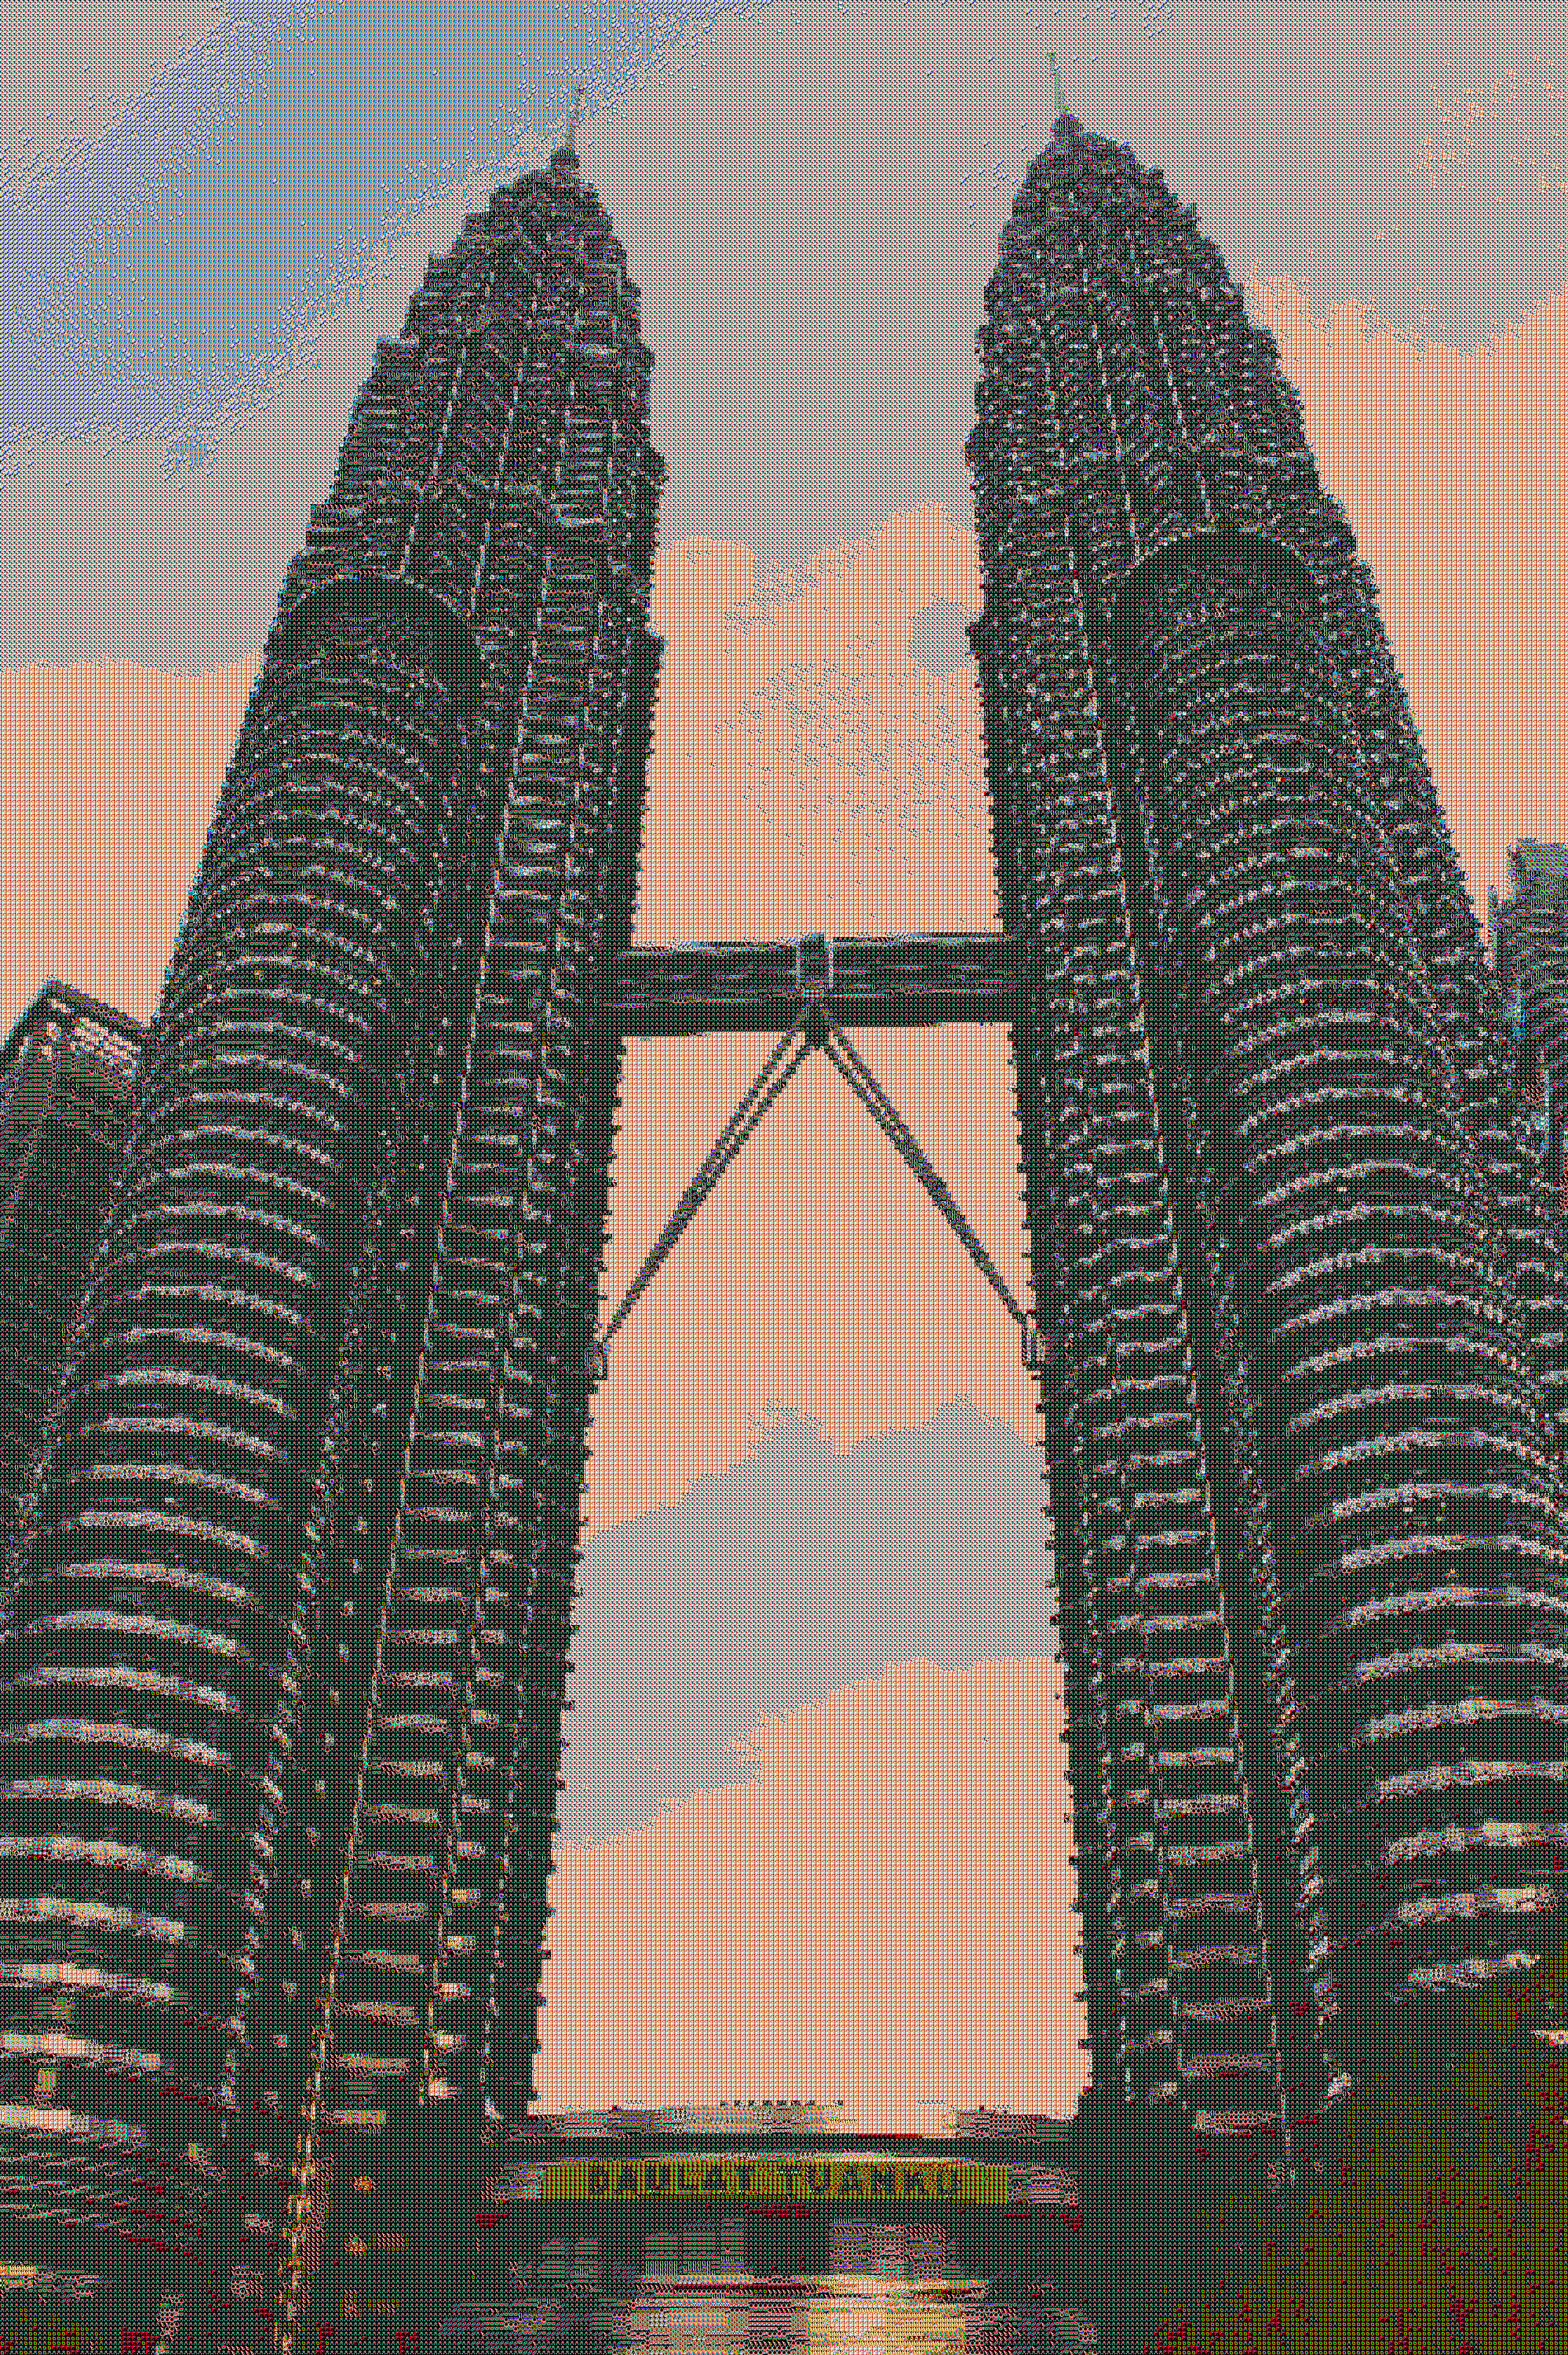
\includegraphics[width=7cm]{output_example.png} }}
    \caption{Comparision between input image and a result example}
    \label{fig:example}%
\end{figure}

In order to the this project through, the very first step is to create a rough design of the application.

\section{Prototype}
\subsection{First draft}

In this part will be prensente the very first design of the application, and the thought process behind. Although its besign might not be the one use for the final version of the software, the concept will stay the same.
Below is presented the above mentioned design: 


\begin{figure}[H]
	\centering
	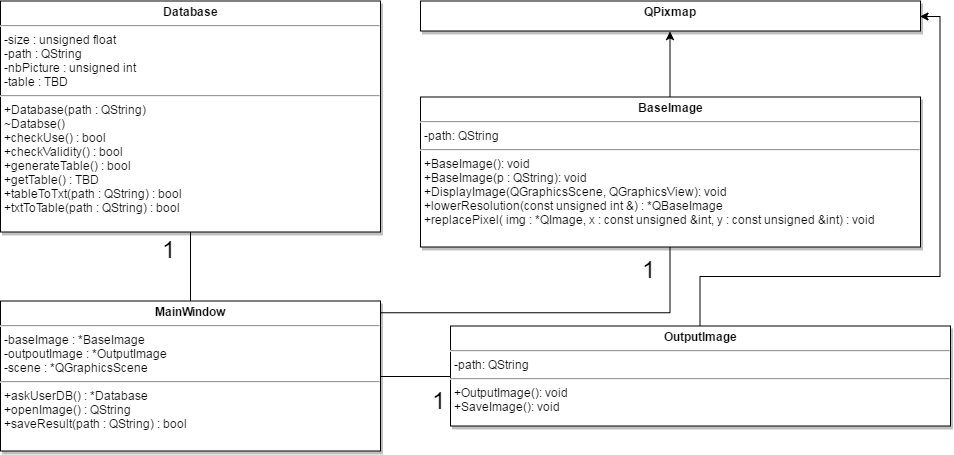
\includegraphics[width=15cm]{First_UML.png}
	\caption{First application design using UML notation}
	\label{fig: FirstUML}    
\end{figure}

Here are the main parts of this UML diagram :

\begin{itemize}
  \item MainWindow, being the core of the application. Handles: GUI, display methods, load and save;
  \item DataBase, being the class handling the image folder selected by the user. From a given path, should be able to load every and only images, and process them;
  \item BaseImage, inherited from QPixmap, being the type used to represent any image loaded into the software. This class conatins the functions to process the images, as well as the reults of these functions;
  \item OutputImage, inherited from QPixmap, containing the image to be saved as well as the methods to perform the save.
\end{itemize}

This UML representation of the project is only the first step, and the diagram is not complete at this point of the development. 
Lets now take a look at the implementation of the finished prototype class by class.

\subsection{BaseImage}
This class is used to represent any image loaded in the software. It contains a set of private variables:

\begin{lstlisting}[language=C++]{Name=BaseImage}
private:
    QString path;
    QColor *mean;
    QImage *image;
    QImage *lowImage;
\end{lstlisting}

The class is holding the basic input image \textit{image} of type \textit{QImage} as well as its \textit{path}, the pixelized version \textit{lowImage} of this image, and finally the \textit{mean} RGB value of the \textit{lowImage}.

This class is equipped with accessors and mutators for each private variable, and also with two functions:

\begin{lstlisting}[language=C++]
public:
    void lowerResolution(const int &);
    void computeMean();
\end{lstlisting}

Following is shown the code of the \textit{BaseImage:lowerResolution(const int \&)} function:
 
\begin{lstlisting}[language=C++]
void BaseImage::computeMean(){
    // Computes the mean value of lowImage

    // get image size
    int h = lowImage->height();
    int w = lowImage->width();

    // init counters in RGB
    int totalR = 0;
    int totalG = 0;
    int totalB = 0;

    // Goign through the image
    for ( int i = 0; i < w; i++){
        for ( int j = 0; j < h; j++){

            // get the current pixel value
            QColor currentpixel( lowImage->pixel( i, j));

            // add the corresponding channels
            totalR += currentpixel.red();
            totalG += currentpixel.green();
            totalB += currentpixel.blue();
        }
    }
    // division to get the mean.
    totalR /= h * w;
    totalG /= h * w;
    totalB /= h * w;
    // creating the resulting color as a qRGB
    setMean(new QColor( totalR, totalG, totalB));
}
\end{lstlisting}

This function is the basic mean fucntion: it goes through each pixel of the image, retrieve its RGB value, add the value of each channel to a counter. Once done, each coutner is divided by the number of pixels in the image, and finally, a dynamic instance of a \textit{QColor} is created to hold the mean (and returned).
This function execution time is clearly depends on the image size and cannot be reduced, unless an approximative mean is calculated, by taking in account only one pixel out of four, for example.

The second function is the \textit{BaseImage::lowerResolution(const int \&ImageSize)} function.
 
\begin{lstlisting}[language=C++]
void BaseImage::lowerResolution(const int &ImageSize)
{
    
     // Lower the resolution of the image by using the average method. The square defined by newH and newW will by applied
    // iteratively on the image, and calulate the mean of the submatrix below this filter. The result is then used to create a pixel in
    // a brand new QImage named lowImage. The spatial organisation of each pixel is kept. In order to fix the boundaries problem,
    // this function just ignores the right and bottom pixel which cannot fit in the filter.

    // get image size
    int h = image->height();
    int w = image->width();
    
    // create a new image with set size according to base image size and mask size
    lowImage = new QImage( int( w / filterSize), int( h / filterSize), QImage::Format_RGB32);
    
    // parsing the image with the filter. placing the top left pixel of the filter on the top left pixel of the image.
    // The filter is then moved regarding newW and newH
    for ( int i = 0; i <= w - filterSize; i = i + filterSize){
        for ( int j = 0; j <= h - filterSize; j = j + filterSize){
        
            // Init the mean variable for this iteration
            int totalR = 0;
            int totalG = 0;
            int totalB = 0;
            
            // looping insinde the resulting submatrix
            for ( int k = i; k < i + filterSize; k++){
                for ( int l = j; l < j + filterSize; l++){
                
                    // get the color of the current pixel
                    QColor currentpixel(image->pixel(k,l));
                    
                    // add the corresponding channels
                    totalR += currentpixel.red();
                    totalG += currentpixel.green();
                    totalB += currentpixel.blue();
                }
            }
            
            // division to get the mean
            totalR /= filterSize * filterSize;
            totalG /= filterSize * filterSize;
            totalB /= filterSize * filterSize;
            
            // creating the resulting color as a qRGB
            QColor result = qRgb( totalR, totalG, totalB);
            
            // create on the new image the resulting pixel
            lowImage->setPixel( int( i / filterSize), int( j / filterSize), result.rgb());
        }
    }
}
\end{lstlisting}

The principle of this function is taking as parameter the size of the filter. If the filter size is set at 20 (for example), a 20-by-20 filter is considered. This filter is moved on the image (first double for loop), and each time it moves, the mean of the pixels below the matrix is computed.This mean RGB value is then used to create, on a brand new image, a new pixel with the mean as a color.
This allow to create a pixelized version of \textit{image}. The result is stored directlty in the class attribute \textit{lowImage}. This function does not address the boundaries problem: it just skips it. Meaning that there is data loss on the rightmost and bottom boudaries, and that images with smaller size than the selected mask can not be used.
The execution time of this function might be problematic. In fact, the implementation is done with 4 inner loops. Meaning that the the size of the image and the size of the filter are not multiplicative between each other, but have a power relation.

\subsection{ImageDB}
This class contains the informations about the image database. The class has been renamed from the UML to avoid any protected keyword conflict.ImageDB

\begin{lstlisting}[language=C++]
private:
    QString path;
    int nbImg;
    std::vector< BaseImage* > data;
\end{lstlisting}

\begin{itemize}
  \item \textit{path}, being the path of the database folder;
  \item \textit{nbImg}, being the number of images in this database;
  \item\textit{data}, being a vector (STL) containing pointers to \textit{BaseImage}. It contains all the instances (pointers to) of the images load into the database.
\end{itemize}

Once again, the class is equipped with getters and setters for each attribute.
Overall, the database has been simplified from its UML model. It now contains two important fucntions: 

\begin{lstlisting}[language=C++]
public:
    void buildDB(const int &);
    BaseImage* bestMatch(const QColor &);
\end{lstlisting}

The \textit{ImageDB::bestMatch(const QColor\&)} function is an optimization function based on the tri-channel mean absolute total difference.


\begin{lstlisting}[language=C++]
BaseImage* ImageDB::bestMatch(const QColor& color)
{
    // Try to find the best match in the DataBase given a color
    // Base on the mean absolute difference otpimisation fucntion

    // Counters for RGB and Total
    int diffR, diffG, diffB, diffT;

    // Base score, 3 channels, max 255/channel
    int opti = 255 * 3;

    // best result
    BaseImage* best;

    // Parse the vector
    for (std::vector<BaseImage*>::iterator it = data.begin(); it != data.end(); it++) {

        // Get current item
        BaseImage* currentImg = *it;

        // Compute the absolute mean difference
        diffR = abs(color.red() - currentImg->getMean()->red());
        diffG = abs(color.green() - currentImg->getMean()->green());
        diffB = abs(color.blue() - currentImg->getMean()->blue());

        // Total mean absolute difference
        diffT = diffR + diffG + diffB;

        // Check if new best result
        if (diffT < opti) {
            best = currentImg;

            // Update best goal
            opti = diffT;
        }
    }
    return best;
}
\end{lstlisting}

This function take as input a \textit{QColor}, which is the value of the pixel in the pixelized base image to replace. The function is looking into \textit{data} to find the best match. The initial score is set at 255 * 3, being the maximum total difference possible between a pixel color and an image mean value (comparing black and white). Then, each instance of \textit{BaseImage} contained in data is compared to the input color by performing the absolute total mean difference. If the result is better than the current best score, then the image is stored as the best one, and the goal score is updated. Finally, the function return the pointer to the best match for the given \textit{QColor}.
This function execution time should be minor. It depends only on the database size, and perform for each instance simpel computations.

The next function is the \textit{ImageDB::buildDB(const int \&)} function.

\begin{lstlisting}[language=C++]
void ImageDB::buildDB(const int& size)
{
    // Instanciate images contained in dir into the vector data, while performing image
    // scaling.

    // source :http://stackoverflow.com/questions/36005814/load-images-from-folder-with-qt
    // StackOverflow, User : Apin, Date : Mar 15 2016

    QDir dir(path);
    QStringList filter;
    filter << QLatin1String("*.png");
    filter << QLatin1String("*.jpeg");
    filter << QLatin1String("*.jpg");
    dir.setNameFilters(filter);
    QFileInfoList filelistinfo = dir.entryInfoList();
    QStringList fileList;
    setNbImg(filelistinfo.size());
    // END OF SOURCE

    // Go through every file
    data.clear();
    foreach (const QFileInfo& fileinfo, filelistinfo) {

        // Get file name
        QString filePath = fileinfo.absoluteFilePath();

        // Instanciate
        BaseImage* tmp = new BaseImage(filePath);

        // Lower resolution
        tmp->lowerResolution(size);

        // Compute mean
        tmp->computeMean();


        // Add the BaseImage instance to the vector
        data.push_back(tmp);
    }
}
\end{lstlisting}

The first part of the function allows the user to select a folder, hopefully containing images. The path of each image is then stored in the \textit{filelistinfo}. Each element of this list is then processed as follow:

\begin{enumerate}
  \item Retrieve the image path;
  \item Instanciate a new \textit{BaseImage}, formed with the image;
  \item Pixelize the image using the \textit{lowerResolution(const int \&size)} method of the instance;
  \item Computes the mean value of the pixelized image
  \item Add the instance in \textit{data}
\end{enumerate}

Once this function is executed, the database is fully ready.
The execution cost of this function is to be remembered: is used the two previously mentionned functions from \textit{BaseImage} that are costly. It might be usefull to use threads on this function to split the computation time and cost. If they are used, a progression bar could be used to show the progress to the user.

\subsection{MainWindow and GUI}
In this part, we will first take a look at the GUI design to have, later, a better understanding of the slots.

\begin{figure}[H]
	\centering
	\includegraphics[width=15cm]{global_numbers.png}
	\caption{GUI design with area segmentation}
	\label{fig: GlobalDesignNumbers}    
\end{figure}

The GUI is organized as follow:

\begin{enumerate}
  \item \textbf{Menu}: Allows the user to load an image, save the final result and quit the program. Each choice can be directly accessed using the appropriate shortcut;
  \item \textbf{QGraphicsView}: This is the area where images are displayed. The first image that is displayed is the basic image loaded by the user. Followd its pixelized version, and finally the artified version of the image;
  \item\textbf{Lower Resolution Button}: Once an image is loaded by the user, this button is enabled (disabled by default). On click, it the image will be pixelized and displayed;
  \item \textbf{Load Database Button}: Becomes enable after the \textbf{Lower Resolution Button} is used. Open a dialog window to allow the user to select a folder containing images. Using this button enable the following one;
  \item \textbf{Process Button}: Once the both the pixelized version of the input image and the database are set, the user can use this button to artify the image.
  \item \textbf{Image Size}: Allows the user to select the number of pixel used to form the pixelized version of the base image. This number is bounded between 10 and 500.
  \item \textbf{SubImage Size}: Allows the user to select the number of pixel used to form the pixelized version of the database images. This number is bounded between 5 and 50.
  \item \textbf{Verbose Console}: This area is visible or not depending on the value of the checkbox named \textit{verbose}. It allows the user to have a feedback on the software status.
\end{enumerate}
Most of these area are defined by slots. Only the interesting parts of it will be presented, as they are either easy to code either redundant.

The \textit{MainWindow} is the centerpoint of the project. Therefore, it contains pointers to other members:

\begin{lstlisting}[language=C++]
private:
    int ImageSize = 50;
    int subImageSize = 30;
    Ui::MainWindow *ui;
    QGraphicsScene *scene;
    BaseImage *baseImg;
    ImageDB *DB;
    BaseImage *result;
    QPlainTextEdit *csl;
\end{lstlisting}
 
 The first thing to see is that the result is not held in a specific class but consider and a \textit{BaseImage}. The \textit{MainWindow} is handeling the save method. 
 Besides the slot functions, this class is equipped with two methods.
 
The first one is the display method named \textit{MainWindow::DisplayImg(QImage *img)}, with the very usual implementation to display a QImage (or in this case QPixmap) using a QGraphicsView and a QGraphicsScene. The only interesting point here is the \textit{void QGraphicsView::fitInView(const QRectF \&rect, Qt::AspectRatioMode aspectRatioMode = Qt::IgnoreAspectRatio)} function, allowing the display of the image so that it fits the area design for this effect, while keeping its aspect ratio.

The secod method is the \textit{void MainWindow::Artify()} method. This method is called when the \textbf{Process Button} is pressed. The function is presented below:

\begin{lstlisting}[language=C++]
void MainWindow::Artify()
{
    // Replace every pixel in baseImg->lowImage by an image in DB which is the best match

    // Retreive the image
    QImage* low = baseImg->getlowImage();

    // get Width and Height
    int h = low->height();
    int w = low->width();


    // best result for a given pixel initialization
    BaseImage* bestResult ;

    // Prepare the result image with good size
    QImage* res = new QImage( baseImg->getlowImage()->width() * subImageSize, baseImg->getlowImage()->height() * subImageSize, QImage::Format_RGB32);

    // for every pixel in the lowImage
    for ( int i = 0; i < w; i++){
        for ( int j = 0; j < h; j++){

            // Get current pixel
            QColor currentpixel(low->pixel( i,j));

            // Get the best result in the DataBase
            bestResult = DB->bestMatch(currentpixel);

            // Get pixelized version
            QImage* pixelized = bestResult->getlowImage();

            // For every pixel in the ebst match low resolution
            for (int k = 0; k< pixelized->width();k++){
                for (int l = 0; l < pixelized->height(); l++){

                    // Get current pixel
                    QColor currentMatch =pixelized->pixel(k,l);

                    // Place on res at the good position
                    res->setPixel(i * subImageSize + k, j * subImageSize + l, currentMatch.rgb());
                }
            }
        }
    }
    result = new BaseImage(res);
}
\end{lstlisting}
 
This fucntion is performing the artification of the image. It first creates a brand new image, which size is determined by the pixelized input image size as well as the database pixelized image size.
Then, for each pixel of the base pixelized image, the best match is the database is found. This match is retrieved, and printed onto the output image at the good position.
Once all the base pixelized image pixels are process, the outut image is finished: the input image has been artified. 
This function execution time relies on several parameters. First, the database size. The whole database is parsed for every pixel in the base image pixeled version. Bringing to the second point: the base image pixelized version size. The more pixel there is, the more is needed processing time. Finally, the SubImage size is important as well, as this image needs to be copied.
So depending on those parameters, the execution time can be instentaneous or quite long.

\subsection{Results}
This prototy allows to reach the final goal. The image presented in Figure.1 at the beginning of this reports shows an example of result. However, after several test, one major problem emerged.
Although the software was perfectly running on small images (2000 images, 60*60 pixels), it was not able to run on a big database (i.e. database with numerous HD images). The code has been modified in many ways to identify the problematic part, which happends to be the \textit{BaseImage} class design.
In fact, to memory allocation for the program upon generating the database explodes. If the step of pixelizing each image and computing the mean are skipped, the software can handle maximum 300 HD images, for a cost of 1.2Go of RAM, which is enormous. It is also interesting to point out that the database generation (only loading images, no other processing) is pretty fast at this stage: about 6 seconds on an average price computer (this data is given just for understanding purposes, the goal is not to estimate the algorithms' complexity). If, in addition of the database iamges instanciation is added the pixelization or the mean (therefore run of the non-pixelized image), the software can not handle the amout of data, leading to a critical failure.
After a lot of work on the \textit{BaseImage} class, it appeared that its design is was really poor, and that major changes needed to be done. Leading to the second iteration of the project.

\section{Second iteration and final software}
\subsection{New design}
in this second version if the project, the \textit{BaseImage} class is removed, leading to a new UML design:

\begin{figure}[H]
	\centering
	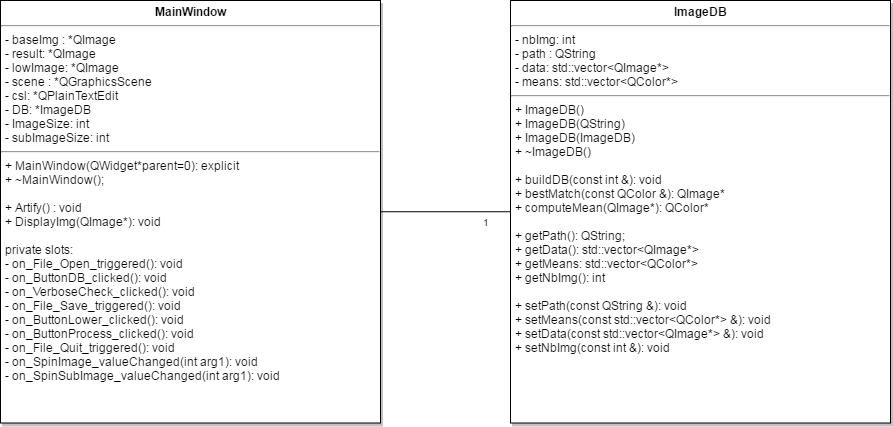
\includegraphics[width=15cm]{Final_UML.png}
	\caption{First application design using UML notation}
	\label{fig: FirstUML}    
\end{figure}

This design is exhaustive: it accuretely represents the code implementation.

There are several design choices that can be pointed out:

\begin{itemize}
  \item Instead of being instanciated under \textit{BaseImage}, all the images are directly treated as \textit{QImage}, as this class provides all the tools needed;
  \item The \textit{computeMean()} function has been move to the \textit{ImageDB} class, as its mother class has be removed;
  \item The means are stored in a vector of QColors, with the same indexing order as the \textit{data} vector;
  \item The \textit{data} vector will now contain the pixelized version of each database image.
\end{itemize}

\subsection{Final implementation}
The removal of the \textit{BaseImage} class led to major restructurion of the methods definitions. Therefore, instead of modifying every definition one by one, a brand new program is has been created. The goal of this fresh start is to keep everything simple and mandatory, while trying to identify which variable should be allocated in the heap or in th stack.
One major change is done on the \textit{ImageDB::buildDB()} fucntion:


\begin{lstlisting}[language=C++]

void ImageDB::buildDB(const int \&size)
{
    // Instanciate images contained in dir into the vector data, while performing image
    // scaling.

    // source :http://stackoverflow.com/questions/36005814/load-images-from-folder-with-qt
    // StackOverflow, User : Apin, Date : Mar 15 2016

    QDir dir(path);
    QStringList filter;
    filter << QLatin1String("*.png");
    filter << QLatin1String("*.jpeg");
    filter << QLatin1String("*.jpg");
    dir.setNameFilters(filter);
    QFileInfoList filelistinfo = dir.entryInfoList();
    QStringList fileList;
    setNbImg(filelistinfo.size());
    // END OF SOURCE

    // Go through every file
    data.clear();
    means.clear();
    foreach (const QFileInfo& fileinfo, filelistinfo) {

        // Get file name
        QString filePath = fileinfo.absoluteFilePath();

        QImage tmp(filePath);

        // Generate pixelized version
        QImage *low = new QImage(tmp.scaled(size,size, Qt::KeepAspectRatio));

        // add data to vector
        data.push_back(low);
        means.push_back(computeMean(low));
    }
}
\end{lstlisting}

We can see that every load image is instanciated in the scope of the function only. In fact, it is used solely to generate its own pixelized verion, which is usefull. This implementation choice is saving a lot of memory, especially for HD images, wich are therefore affecting only the pixelization process time.
This change by itself brings the total memory load (pixelized image instance + QColor to hold the mean)  at 67Mb for a 300 HD images database. Although, it appears taht the processing time has changed. In fact, while the number of operations has been reduced with this design, the processing time is highly increased. After some investigation, the source of this computation time increase is still unknown. Some thoughts and tries were given to QThread an useual C++ threading methods, but the development team (i.e. myself) is a bit rusty on those technicalities. This problem could be addressed in a later iteration of the software.

The other change is due to the discovery (not of fire, but still close) of the function \textit{QImage QImage::scaled(int width, int height, Qt::AspectRatioMode aspectRatioMode = Qt::IgnoreAspectRatio, Qt::TransformationMode transformMode = Qt::FastTransformation) const}, which single handedly perfomes the pixelization, with no `data loss' (boundary effect). It has been use as replacement for the now old \textit{BaseImage::lowerResolution()}. 

Overall, the code has been improved, by being minimalist yet complete. Optimization has been considered and applied regarding methods parameters. 

\subsection{Results}
The software is now able to run on any database, and has been tested for `dumb-user issue' in some cases, but not exhaustivly (no sanity check on the database content). A normal use of the software (guideline could be the numbers on the GUI presentation) should not lead to any critical or functionnal error. 
The program can be used with any input image of type .png, .jpg and .jpeg, and also with any database: every user can use its most favorite pictures. The result is always saved under the .png format.

Even though the software is not perfect, it has been deployed, to allow its use outside of conception mode. The deployed version can be found on  \href{https://github.com/AntoineMerlet/ProjectCXX/blob/master/Deploy.zip}{my Github}. A personne willing to use the sofware by herself could use the sample images provided on the same github to have a database (the author does not own any of these images).

In order see the output image of the software, i would recommand the user to try it by himself. If fact, the results can niot be shown properly in such a report, as there size is enormous. Alternatively, some results are avialable on my github repository.


\section{Conclusion}
This project is somewhat sucesseful. Even though some minor issues needs to be addressed (`dumb-user' sanity checks), the software can be used to artify an image, by replacing its pixels with images.
Once more, the author of the project had the opportunity to realize that a bad design is sometime worse than no design. The implementation of the first prototype took several hours, while the design and the implementation of the final version took about 3 hours.
The project helped a lot to get used again to the Qt documentation, as well as propoer code writting (there is still some work to do here).
The author is satisfied with the output that the software is producing. However, this project could have been done way faster with proper project management and methodic coding habits(commits/comments).  
 

\begin{figure}[H]
	\centering
	\includegraphics[width=15cm]{condorcet.png}
	\caption{Our beautiful university}   
\end{figure}

\end{document} % DONE WITH DOCUMENT!


%https://www.generationrobots.com/fr/401271-turtlebot-2-robot-mobile-ros.html
